\documentclass[conference]{IEEEtran}
\IEEEoverridecommandlockouts
\usepackage[spanish]{babel}
\usepackage{amsmath,amssymb,amsfonts}
\usepackage{graphicx}
\usepackage{array}     % columnas p{} con \raggedright, para evitar cajas underfull
\usepackage{textcomp}
\usepackage{listings}
\usepackage{xcolor}
\usepackage{float}
\usepackage{tcolorbox}
\usepackage{eso-pic}
\usepackage{transparent}
\usepackage{hyperref}  % debe cargarse de último para no duplicar anclas de floats

\pagestyle{plain}

% Los flotantes a doble columna (figure* y table*) de este informe son grandes:
% se amplía el espacio que pueden ocupar en la parte superior de la página para
% que no se acumulen ni se desplacen lejos del texto que los cita.
\renewcommand{\topfraction}{0.92}
\renewcommand{\textfraction}{0.06}
\renewcommand{\floatpagefraction}{0.72}
\renewcommand{\dbltopfraction}{0.92}
\renewcommand{\dblfloatpagefraction}{0.72}
\setcounter{topnumber}{3}
\setcounter{dbltopnumber}{3}
\setcounter{totalnumber}{5}

\newif\ifshowwatermark
\showwatermarktrue
\AddToShipoutPictureBG{%
    \ifshowwatermark
        \AtPageCenter{%
            \makebox(0,0){%
                \transparent{0.18}%
                
\includegraphics[width=1.0\textwidth]{assets/images/Logo}%
            }%
        }%
    \fi
}

\lstset{
    columns=fullflexible,
    basicstyle=\ttfamily\scriptsize\color[RGB]{30,30,30},
    keywordstyle=\bfseries\color[RGB]{0,90,160},
    commentstyle=\itshape\color[RGB]{100,100,100},
    stringstyle=\color[RGB]{160,60,0},
    numberstyle=\tiny\color[RGB]{150,150,150},
    numbers=left,
    numbersep=8pt,
    stepnumber=1,
    backgroundcolor=\color[RGB]{248,248,252},
    frame=none,
    showstringspaces=false,
    breaklines=true,
    breakatwhitespace=false,
    % Sin esto, la continuación de una línea partida se alinea con la sangría
    % original; en el código de Plotly, con sangrías de más de 50 columnas, eso
    % desborda la caja. Se parte al margen izquierdo del bloque.
    breakautoindent=false,
    breakindent=0pt,
    tabsize=4,
    captionpos=b,
    xleftmargin=15pt,
    xrightmargin=5pt,
    inputencoding=utf8,
    extendedchars=true,
    literate=
        {á}{{\'a}}1 {é}{{\'e}}1 {í}{{\'i}}1 {ó}{{\'o}}1 {ú}{{\'u}}1
        {Á}{{\'A}}1 {É}{{\'E}}1 {Í}{{\'I}}1 {Ó}{{\'O}}1 {Ú}{{\'U}}1
        {ñ}{{\~n}}1 {Ñ}{{\~N}}1
        {°}{{\textdegree}}1
        {σ}{{$\sigma$}}1
        {≈}{{$\approx$}}1
        {¨}{}1
        {—}{{---}}1
        {–}{{--}}1
        {·}{{\textperiodcentered}}1
        {×}{{$\times$}}1
        {−}{{$-$}}1
        {²}{{$^{2}$}}1
        {Δ}{{$\Delta$}}1
        {√}{{$\surd$}}1
        {ŷ}{{$\hat{y}$}}1
        {¿}{{\textquestiondown}}1
}

% Estilos por lenguaje: Python para el cálculo principal y R para la
% verificación cruzada, ambos sobre la misma identidad visual.
\lstdefinestyle{python}{
    language=Python,
    morekeywords={np, plt, pd, ax, ax1, ax2, axes, fig, Path},
}

\lstdefinestyle{rlang}{
    language=R,
    morekeywords={png, dev, par, grid, abline, barplot, boxplot, legend, text,
                  points, lines, hist, sapply, tapply, cumsum, seq, sprintf},
}

\lstset{style=python}

\def\BibTeX{{\rm B\kern-.05em{\sc i\kern-.025em b}\kern-.08em T\kern-.1667em\lower.7ex\hbox{E}\kern-.125emX}}

\renewcommand{\refname}{Referencias}

\addto\captionsspanish{%
    \renewcommand{\tablename}{Tabla}%
    \renewcommand{\lstlistingname}{Código}%
}

\begin{document}
    \raggedbottom
    \bstctlcite{IEEEtran:BSTcontrol}

    \title{
        Análisis de regresión y visualización avanzada del consumo energético:
        del diagnóstico de supuestos a la validación predictiva
    }

    \author{\IEEEauthorblockN{
        Andrés Giovanny Rubiano Muñoz ``Andy Rubiano''}
        \IEEEauthorblockA{
            \textit{Maestría en Inteligencia Artificial, Facultad de Ingeniería} \\
            \textit{Universidad de La Salle} \\
            Bogotá, Colombia \\
            arubiano67@unisalle.edu.co
        }
    }

    \maketitle
    \thispagestyle{plain}

    \begin{abstract}
        Una recta que explica el 99,7\% de la variabilidad parece un resultado
        difícil de mejorar, pero este informe muestra que ese número, por sí solo,
        no dice si el modelo es correcto. Sobre el consumo energético mensual de 120
        clientes de los sectores residencial, comercial e industrial se estima una
        regresión simple que alcanza un coeficiente de determinación de 0,9969 y aun
        así rechaza la homocedasticidad y la normalidad de sus residuos, que no son
        ruido sino que se ordenan por sector, con medias de $-4{,}4$, $+15{,}5$ y
        $-19{,}2$ miles de pesos. Que la prueba RESET no rechace señala que el
        problema no es la forma funcional sino una variable omitida, por lo que se
        incorpora el sector y su interacción con el consumo. Las pendientes del
        modelo resultante tienen nombre propio, pues son las tarifas de cada sector
        (791,6, 704,8 y 671,0 pesos por kilovatio hora) y reproducen con menos del
        4\% de diferencia el cociente entre costo y consumo calculado sin
        intervención del modelo. La mejora se sostiene fuera de la muestra, ya que la
        validación cruzada de diez pliegues reduce el error un 16,7\% y sobre 36
        clientes no vistos alcanza un coeficiente de determinación de 0,9944 con un
        error porcentual absoluto medio del 3,68\%. La verificación cruzada en R
        reproduce los seis coeficientes dígito a dígito, y el descuento por escala
        queda cuantificado en 121 pesos por kilovatio hora entre el sector
        industrial y el residencial.
    \end{abstract}

    \vspace{10pt}

    \begin{IEEEkeywords}
        Criterios de información, diagnóstico de supuestos, ggplot2, Plotly,
        regresión lineal múltiple, scikit-learn, seaborn, statsmodels, validación
        cruzada, visualización avanzada.
    \end{IEEEkeywords}

    \section{Introducción}
    Una recta que explica el 99,7\% de la variabilidad de los datos parece un
    resultado difícil de mejorar. Este informe muestra que ese número, por sí solo,
    no dice si el modelo es correcto, dado que la misma regresión que alcanza un
    coeficiente de determinación de 0,9969 deja residuos que no son ruido, sino que
    se ordenan según una variable que quedó fuera del modelo. Detectar esa
    estructura, incorporarla y verificar que el modelo corregido cumple los
    supuestos que sostienen su inferencia es el recorrido completo de un análisis de
    regresión \cite{montgomery2021regression}, \cite{wooldridge2020econometrics}, y
    es también el recorrido de este trabajo.

    \vspace{10pt}

    El análisis se apoya en un conjunto de datos simulado del consumo energético
    mensual de 120 clientes de una empresa distribuidora, repartidos en los sectores
    Residencial, Comercial e Industrial. Que el conjunto sea simulado es una ventaja
    metodológica y no una limitación, puesto que se sabe de antemano que existen
    tres poblaciones con tarifas medias distintas, de modo que el modelo puede
    evaluarse por su capacidad de recuperar una estructura conocida y no solo por su
    ajuste.

    \vspace{10pt}

    El informe se organiza en dos capítulos. El primero describe la metodología,
    con el conjunto de datos, la secuencia de modelos estimados, las medidas que los
    comparan y el flujo de trabajo reproducible que los produce; el segundo presenta
    los resultados, desde el análisis de correlación hasta la verificación cruzada
    entre Python y R, pasando por el diagnóstico del modelo simple, la especificación
    múltiple, la validación predictiva y la visualización avanzada
    \cite{castro2026avanzada}. Los seis scripts que sostienen el análisis se
    reproducen completos en los Apéndices \ref{anexo_python} y \ref{anexo_r}, de modo
    que cada cifra del informe puede rastrearse hasta la línea que la produce.

    \vspace{10pt}

    Tres hallazgos anticipan el contenido. El primero es que las pendientes del
    modelo múltiple tienen nombre propio, pues son las tarifas de cada sector,
    791,6, 704,8 y 671,0 pesos por kilovatio hora, y reproducen con menos del 4\% de
    diferencia el cociente entre costo y consumo calculado sin pasar por la
    regresión. El segundo es que ese modelo no solo ajusta mejor dentro de la
    muestra, sino que también predice mejor fuera de ella, ya que la validación
    cruzada de diez pliegues reduce el error un 16,7\% frente al modelo simple. El
    tercero es que el sector Industrial paga 121 pesos por kilovatio hora menos que
    el Residencial, un descuento por escala que el análisis cuantifica y que la
    empresa puede contrastar con su política tarifaria.

    \section{Metodología}
    El desarrollo se implementó en dos scripts independientes que se ejecutan con orden
    incremental, puesto que cada paso depende del anterior, iniciando con la preparación
    del entorno, siguiendo con la generación del conjunto de datos, la construcción de la
    distribución de frecuencias por la regla de Sturges, el cálculo de las medidas de
    tendencia central y de dispersión y, por último, la producción de los gráficos
    básicos y su verificación cruzada en R. Ambos scripts se reproducen completos en los
    Anexos \ref{anexo_python} y \ref{anexo_r}, de modo que esta sección describe las
    decisiones de implementación y el lector puede contrastarlas allí línea por línea.

    \subsection{Herramientas y entorno de trabajo}
        Las alternativas disponibles para un laboratorio de estadística descriptiva 
        se agrupan en tres familias, las hojas de cálculo, que ofrecen funciones y 
        gráficos inmediatos pero mezclan datos, fórmulas y resultados en un mismo 
        lienzo y dificultan auditar los cálculos y reproducirlos sobre datos nuevos
        \cite{toro2022ciencia}, \cite{timbers2024datascience},
        \cite{castro2026cienciadatos}, los entornos de programación científica, que
        expresan cada cálculo como código versionable capaz de regenerar exactamente 
        los mismos resultados y figuras \cite{castro2026visualizacion} y las librerías
        declarativas junto con las plataformas de inteligencia de negocios, que 
        producen gráficos con poco código a cambio de un menor control sobre los 
        elementos que los principios de diseño exigen ajustar \cite{few2012show}.

        \vspace{10pt}

        Se elige la segunda familia con \textit{pandas} y \textit{Matplotlib} como
        herramienta principal por dos razones, la primera es que el cálculo y su
        representación conviven en el mismo script, pues la tabla de frecuencias 
        se obtiene con \texttt{numpy.histogram} \cite{harris2020numpy} y las medidas 
        por grupo con \textit{pandas} \cite{mckinney2010data} y esas mismas estructuras
        alimentan directamente las figuras, eliminando transcripciones manuales que son
        fuente de error, la segunda es que \textit{Matplotlib} otorga el control fino 
        que exige la aplicación de los principios de diseño \cite{hunter2007matplotlib}, 
        ya que permite fijar las clases de Sturges como bordes del histograma, superponer
        las líneas de media, mediana y moda, forzar el eje de frecuencias desde cero o
        situar la cuadrícula detrás de los datos \cite{few2012show}, 
        \cite{castro2026visualizacion}. Como herramienta de contraste se emplea R base, 
        que implementa los mismos cálculos con funciones nativas como \texttt{mean}, 
        \texttt{median}, \texttt{var}, \texttt{sd} e \texttt{hist}, sin dependencias 
        externas \cite{castro2026visualizacion}, \cite{rcore2024r}. La comparación es 
        directa porque \texttt{var()} y \texttt{sd()} de R son muestrales, con divisor 
        $n - 1$, exactamente como el parámetro \texttt{ddof=1} de \textit{pandas}, 
        de modo que los resultados deben coincidir dígito a dígito.

    \subsection{Conjunto de datos}
        Se emplea un conjunto de datos simulado que corresponde al consumo energético
        mensual de 120 clientes de una empresa distribuidora, generado con semilla fija
        (42) para garantizar que las observaciones sean reproducibles y puedan
        regenerarse de manera idéntica en cada ejecución. Los sectores se asignan con
        probabilidades de 0,50 para Residencial, 0,30 para Comercial y 0,20 para
        Industrial, el consumo proviene de distribuciones normales con parámetros
        propios de cada sector y el costo resulta de una tarifa diferenciada con un
        ruido multiplicativo del 4\%. Las variables del dataset se muestran a 
        continuación:

        \begin{table}[H]
            \centering
            \caption{Variables del conjunto de datos}
            \begin{center}
                \begin{tabular}{|l|l|>{\raggedright\arraybackslash}p{3.1cm}|}
                    \hline
                    \textbf{Variable} & \textbf{Tipo} & \textbf{Descripción} \\
                    \hline
                    cliente\_id & Nominal & Identificador único del cliente
                    (CL-001 a CL-120) \\
                    \hline
                    sector & Nominal & Residencial, Comercial o Industrial \\
                    \hline
                    consumo\_kwh & Cuantitativa continua & Consumo mensual en
                    kilovatios-hora \\
                    \hline
                    costo\_miles\_cop & Cuantitativa continua & Facturación mensual en
                    miles de pesos colombianos \\
                    \hline
                \end{tabular}
                \label{dataset_variables}
            \end{center}
        \end{table}

        El carácter simulado del dataset constituye una ventaja metodológica para este
        laboratorio, puesto que al conocerse de antemano que existen tres poblaciones
        con medias separadas, es posible evaluar si cada estadístico y cada gráfico
        revela u oculta esa estructura, explicando con precisión por qué las medidas
        globales difieren tanto de las sectoriales.

    \subsection{Flujo de trabajo y reproducibilidad}
        El flujo inicia en Python (Anexo \ref{anexo_python}), donde \textit{statistics.py} 
        genera el dataset, calcula los estadísticos y exporta los resultados y las 
        figuras en formatos CSV y PNG, posteriormente, R (Anexo \ref{anexo_r}) utiliza 
        el mismo conjunto de datos para recalcular los estadísticos de forma independiente y
        replicar las figuras mediante su graficación base, permitiendo contrastar ambos 
        resultados.

    \subsection{Construcción de la distribución de frecuencias}
        La tabla de frecuencias se construye aplicando la regla de Sturges 
        (ecuación \ref{sturges}) al consumo global para determinar el número de clases, 
        los intervalos, de igual amplitud, se generan con \texttt{numpy.linspace}, 
        mientras que \texttt{numpy.histogram} calcula las frecuencias absolutas para 
        luego obtener las frecuencias acumuladas y relativas y la marca de clase de 
        cada intervalo.

    \subsection{Cálculo de las medidas de tendencia central}
        La media y la mediana se calculan directamente con \textit{pandas}, mientras 
        que la moda, al tratarse de una variable continua, se estima mediante la 
        función \texttt{interpolated\_mode}, adicionalmente, se identifica la clase 
        modal con \texttt{argmax} y aplica la ecuación (\ref{moda_interpolada}), 
        considerando el caso $d_{1}+d_{2}=0$, en el que se utiliza el punto medio 
        de la clase. El procedimiento se repite para cada sector recalculando sus 
        intervalos según la regla de Sturges para adaptarlos al tamaño de cada 
        muestra.

    \subsection{Cálculo de las medidas de dispersión}
        Las medidas de dispersión se calculan con las ecuaciones (\ref{rango}) a
        (\ref{iqr}), fijando de manera explícita \texttt{ddof=1} en la varianza y en la
        desviación estándar para obtener los estimadores muestrales, que son justamente
        los que R implementa por defecto en \texttt{var()} y \texttt{sd()}, condición que
        hace posible la verificación cruzada dígito a dígito.

    \subsection{Verificación cruzada en R}
        El script de R no reutiliza ningún resultado de Python, únicamente lee el 
        archivo CSV con las 120 observaciones y vuelve a calcular desde cero la tabla 
        de frecuencias y todos los estadísticos, de manera que cualquier discrepancia
        revelaría un error de implementación en alguno de los dos entornos; la 
        distribución de frecuencias en R reproduce el mismo procedimiento, generando 
        los bordes con \texttt{seq} y contando con \texttt{hist} en modo silencioso, 
        con el argumento \texttt{include.lowest} activo para que la observación mínima 
        quede dentro de la primera clase, tal como lo hace \texttt{numpy.histogram}, 
        por último, la función \texttt{summary\_stats} condensa en un solo vector las
        ocho medidas de las Tablas \ref{central_tendency} y \ref{dispersion} y se 
        aplica a cada sector y al conjunto global.
    \section{Resultados}
    \subsection{Distribución de frecuencias del consumo}
        Con $n = 120$, la regla de Sturges arroja $k = 8$ clases de amplitud 457,0 kWh
        sobre el recorrido comprendido entre 121,2 y 3.777,1 kWh. Antes de leer las
        frecuencias conviene saber quién ocupa cada clase, pues los tres sectores cubren
        franjas de consumo que apenas se solapan y, en consecuencia, cada clase resulta
        casi de un solo sector, tal como lo detalla la Tabla \ref{class_sector}.

        \begin{table}[H]
            \centering
            \caption{Composición por sector de cada clase de consumo}
            \begin{center}
                \begin{tabular}{|l|c|c|c|c|}
                    \hline
                    \textbf{Clase (kWh)} & \textbf{Resid.} & \textbf{Comer.} &
                    \textbf{Indus.} & \textbf{Clientes} \\
                    \hline
                    [121,2 -- 578,2)     & 62 & 3  & --  & 65 \\
                    \hline
                    [578,2 -- 1.035,2)   & -- & 27 & --  & 27 \\
                    \hline
                    [1.035,2 -- 1.492,2) & -- & 10 & --  & 10 \\
                    \hline
                    [1.492,2 -- 1.949,2) & -- & -- & 5   & 5  \\
                    \hline
                    [1.949,2 -- 2.406,1) & -- & -- & 1   & 1  \\
                    \hline
                    [2.406,1 -- 2.863,1) & -- & -- & 6   & 6  \\
                    \hline
                    [2.863,1 -- 3.320,1) & -- & -- & 3   & 3  \\
                    \hline
                    [3.320,1 -- 3.777,1] & -- & -- & 3   & 3  \\
                    \hline
                    \textbf{Total}       & \textbf{62} & \textbf{40} & \textbf{18} &
                    \textbf{120} \\
                    \hline
                \end{tabular}
                \label{class_sector}
            \end{center}
        \end{table}

        Sobre esas mismas clases se construye la distribución de frecuencias completa que
        se observa en la Tabla \ref{freq_table}.

        \begin{table}[H]
            \centering
            \caption{Distribución de frecuencias del consumo mensual (kWh)}
            \begin{center}
                \begin{tabular}{|l|c|c|c|c|c|}
                    \hline
                    \textbf{Clase (kWh)} & \textbf{Marca} & $\mathbf{f_{i}}$ &
                    $\mathbf{F_{i}}$ & $\mathbf{h_{i}}$ \textbf{(\%)} &
                    $\mathbf{H_{i}}$ \textbf{(\%)} \\
                    \hline
                    [121,2 -- 578,2)     & 349,7   & 65 & 65  & 54,2 & 54,2  \\
                    \hline
                    [578,2 -- 1.035,2)   & 806,7   & 27 & 92  & 22,5 & 76,7  \\
                    \hline
                    [1.035,2 -- 1.492,2) & 1.263,7 & 10 & 102 & 8,3  & 85,0  \\
                    \hline
                    [1.492,2 -- 1.949,2) & 1.720,7 & 5  & 107 & 4,2  & 89,2  \\
                    \hline
                    [1.949,2 -- 2.406,1) & 2.177,6 & 1  & 108 & 0,8  & 90,0  \\
                    \hline
                    [2.406,1 -- 2.863,1) & 2.634,6 & 6  & 114 & 5,0  & 95,0  \\
                    \hline
                    [2.863,1 -- 3.320,1) & 3.091,6 & 3  & 117 & 2,5  & 97,5  \\
                    \hline
                    [3.320,1 -- 3.777,1] & 3.548,6 & 3  & 120 & 2,5  & 100,0 \\
                    \hline
                \end{tabular}
                \label{freq_table}
            \end{center}
        \end{table}

        La concentración en los niveles bajos de consumo es clara, la primera clase reúne
        el 54,2\% de las observaciones y las dos primeras acumulan el 76,7\%, mientras que
        el 10\% de los clientes con consumos superiores a 1.949,2 kWh se reparte en cuatro
        clases. El hueco de la quinta clase, con una sola observación, es la franja vacía
        que separa el techo del sector Comercial del grueso del Industrial. La
        distribución no corresponde entonces a una población única con cola larga, sino a
        tres subpoblaciones de escalas distintas resumidas en una sola tabla, hecho que
        anticipa la brecha entre la media y la mediana globales.

        \vspace{10pt}

        La Figura \ref{hist_sturges} representa la distribución mediante un histograma y 
        superpone las tres medidas de tendencia central, junto con su réplica independiente 
        en R. La posición de estas medidas permite identificar claramente la forma de la 
        distribución, dado que la mediana (378,6 kWh) y la moda interpolada (409,6 kWh) se 
        encuentran próximas entre sí y dentro de la zona de mayor concentración de 
        observaciones, mientras que la media (819,1 kWh) se desplaza considerablemente 
        hacia la derecha debido a los elevados consumos del sector Industrial. Este
        comportamiento evidencia una marcada asimetría positiva, en la que la media, 
        aunque incorpora todas las observaciones, se ve influenciada por los valores 
        extremos y deja de representar adecuadamente el consumo del cliente típico.

        \begin{strip}
            \centering
            \begin{minipage}{0.49\textwidth}
                \centering
                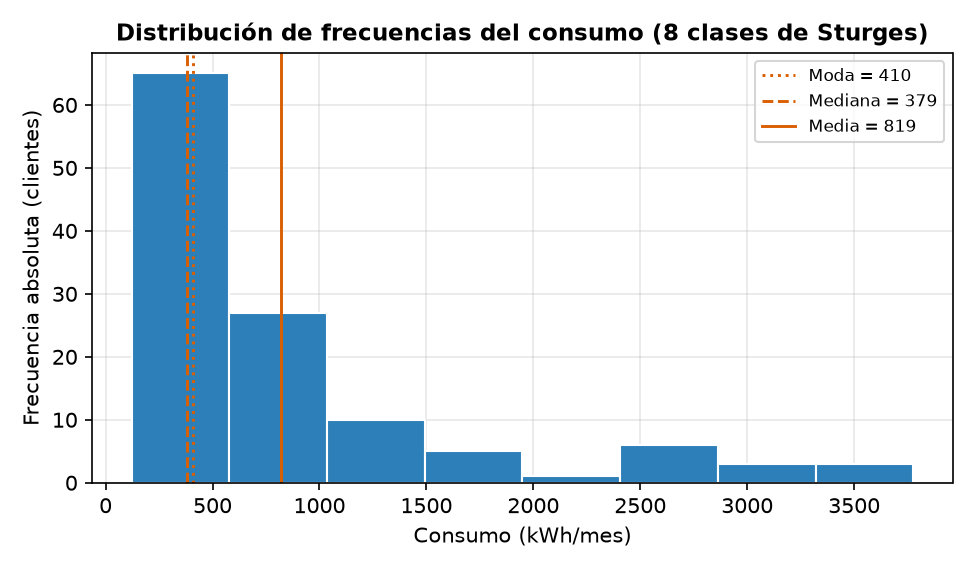
\includegraphics[width=\linewidth]{assets/images/figures/python/hist_sturges_central_tendency.png}
            \end{minipage}
            \hfill
            \begin{minipage}{0.49\textwidth}
                \centering
                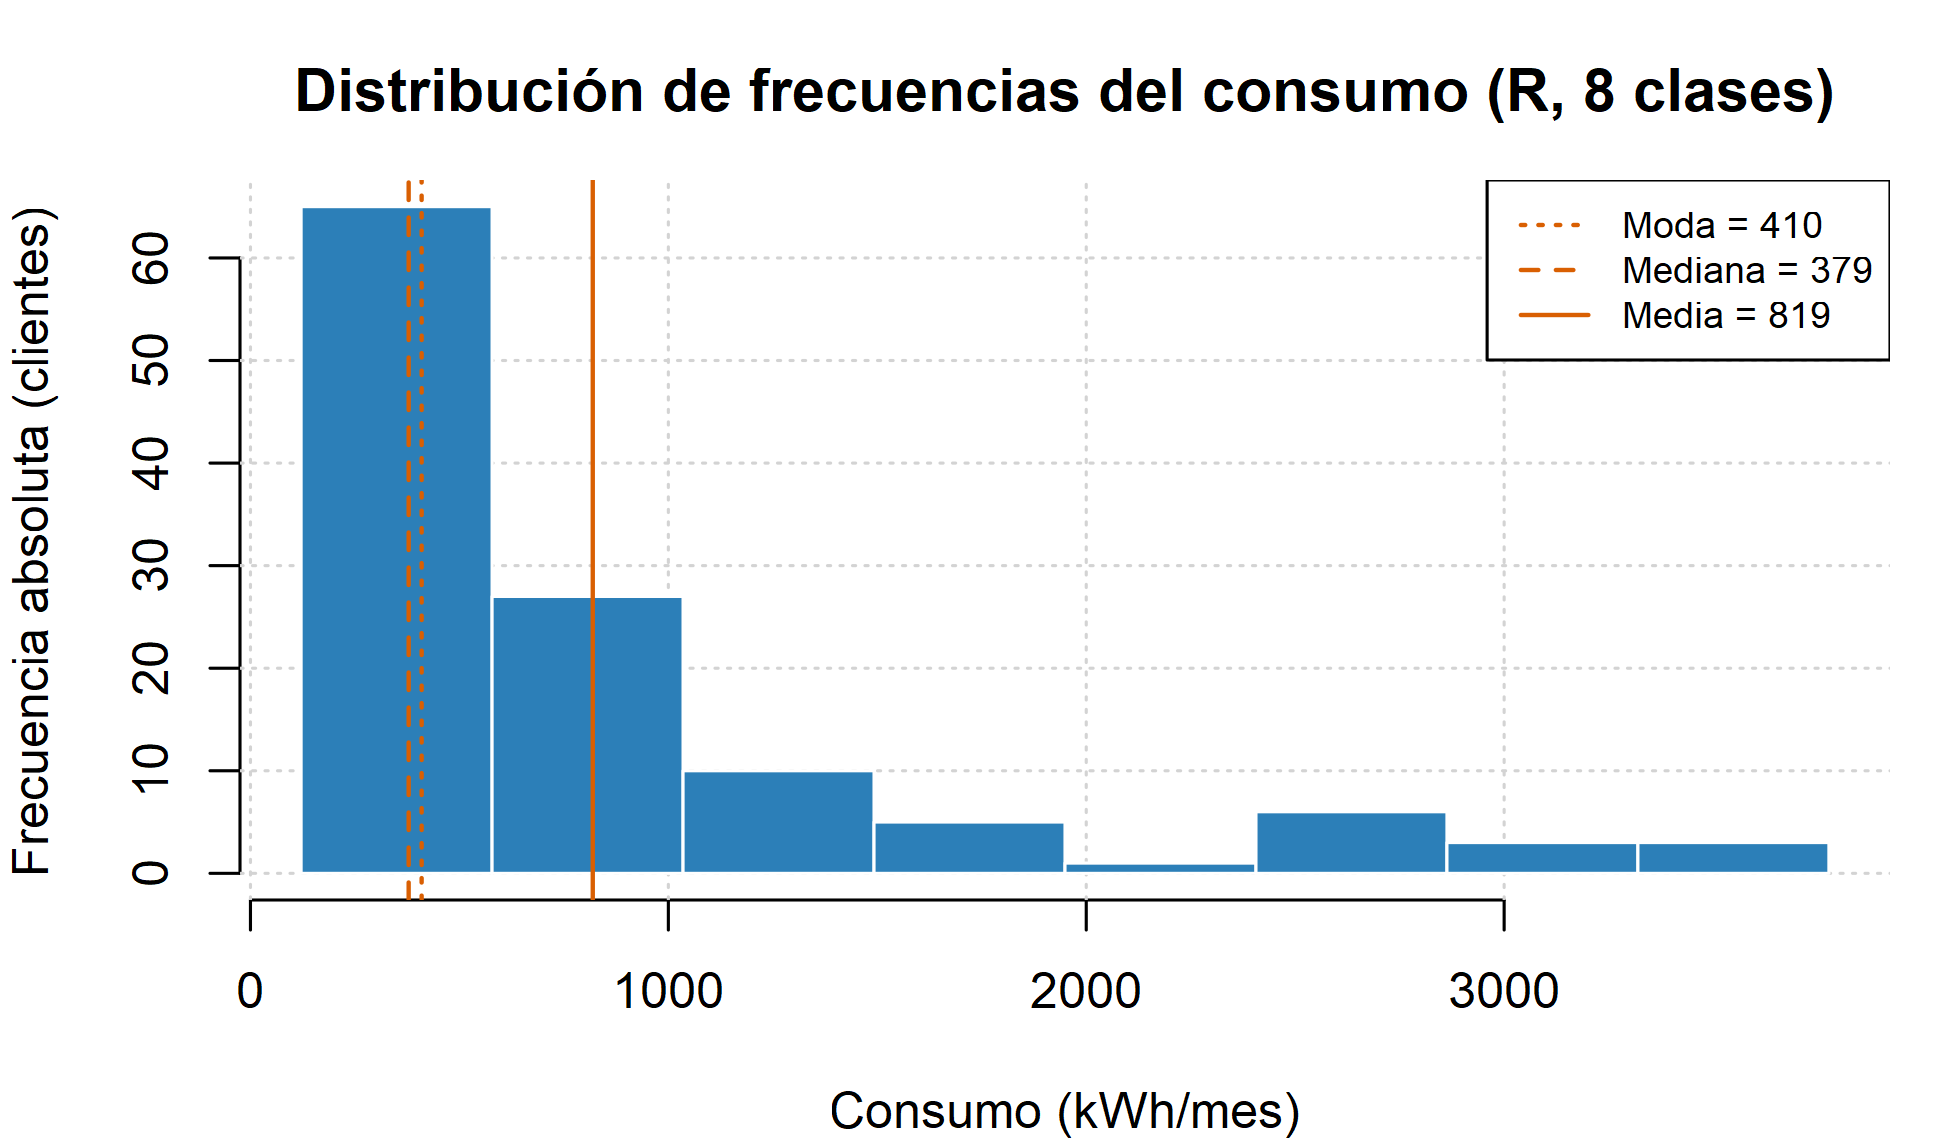
\includegraphics[width=\linewidth]{assets/images/figures/r/hist_sturges_central_tendency.png}
            \end{minipage}

            \vspace{4pt}

            \captionof{figure}{Distribución de frecuencias del consumo mensual con media,
            mediana y moda, en Matplotlib (izquierda) y su réplica en R (derecha)}
            \label{hist_sturges}
        \end{strip}

        La Figura \ref{polygon_ogive} presenta las otras dos representaciones de la
        misma tabla, el polígono de frecuencias y la ojiva, sobre la cual la horizontal
        del 50\% corta la curva en la mediana de aproximadamente 379 kWh. El polígono 
        comunica la misma información del histograma pero enfatiza la tendencia antes 
        que la magnitud de cada clase, mientras que la ojiva convierte la pregunta 
        ``cuántos clientes hay en esta clase'` en ``qué fracción del total queda por 
        debajo de este consumo'', permitiendo leer directamente sobre el eje cualquier 
        percentil, empezando por la mediana.

        \clearpage

        \begin{strip}
            \centering
            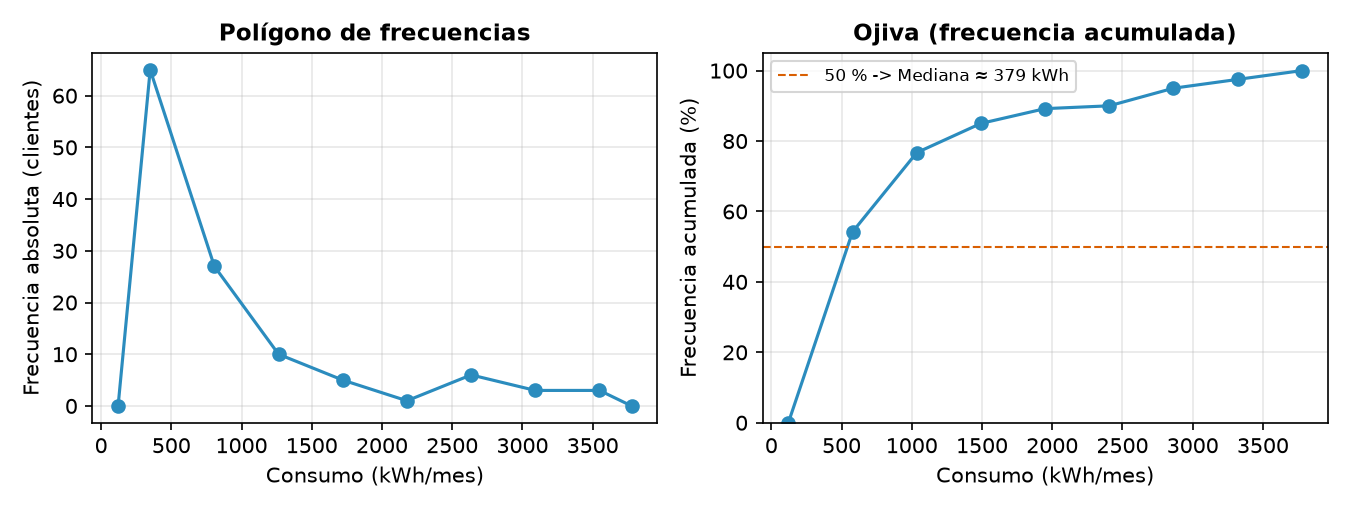
\includegraphics[width=0.86\linewidth]{assets/images/figures/python/freq_polygon_ogive.png}

            \vspace{6pt}

            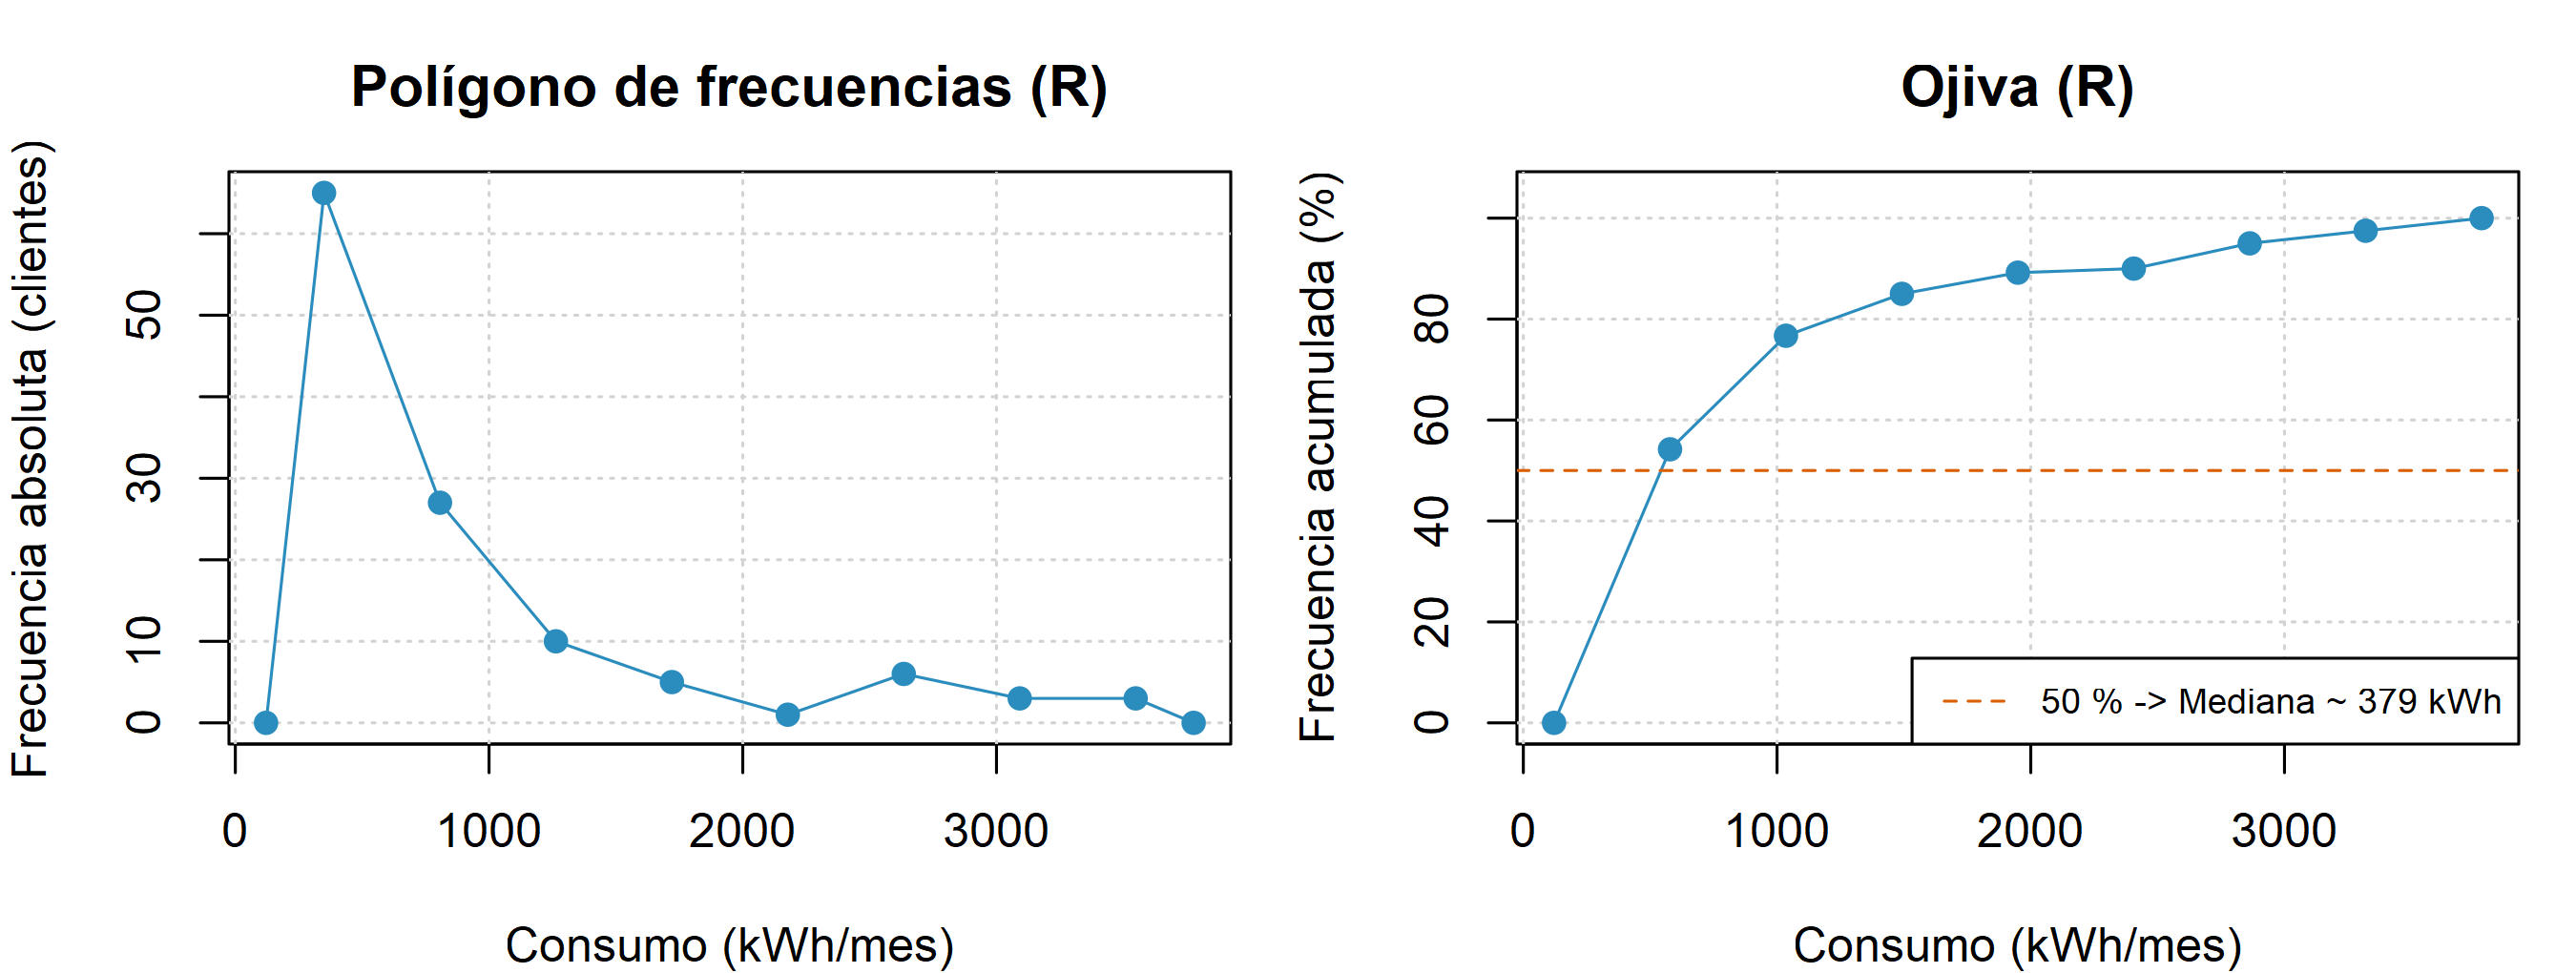
\includegraphics[width=0.86\linewidth]{assets/images/figures/r/freq_polygon_ogive.png}

            \vspace{4pt}

            \captionof{figure}{Polígono de frecuencias y ojiva del consumo mensual, en
            Matplotlib (arriba) y su réplica en R (abajo)}
            \label{polygon_ogive}
        \end{strip}

        La réplica en R exige un detalle de implementación que ilustra los principios de
        visualización, dado que la graficación base dibuja la cuadrícula encima de lo ya
        trazado, por lo que cada figura se construye en dos pasadas, la primera sin
        relleno para fijar los ejes y la escala, luego se inserta la cuadrícula y la
        segunda pasada dibuja los datos por encima, garantizando que la retícula quede
        siempre por detrás.

    \subsection{Medidas de tendencia central}
        La Tabla \ref{central_tendency} presenta la media, la mediana y la moda
        interpolada del consumo por sector y a nivel global. La moda de la variable
        nominal sector es Residencial, con 62 de los 120 clientes, equivalentes al
        52\%.

        \begin{table}[H]
            \centering
            \caption{Medidas de tendencia central del consumo mensual (kWh)}
            \begin{center}
                \begin{tabular}{|l|c|c|c|c|}
                    \hline
                    \textbf{Grupo} & $\mathbf{n}$ & \textbf{Media} & \textbf{Mediana} &
                    \textbf{Moda interp.} \\
                    \hline
                    Residencial & 62  & 248,3   & 240,6   & 232,7   \\
                    \hline
                    Comercial   & 40  & 878,1   & 866,6   & 787,8   \\
                    \hline
                    Industrial  & 18  & 2.654,0 & 2.666,8 & 1.849,3 \\
                    \hline
                    Global      & 120 & 819,1   & 378,6   & 409,6   \\
                    \hline
                \end{tabular}
                \label{central_tendency}
            \end{center}
        \end{table}

        El contraste entre los niveles de la tabla es el hallazgo central del análisis,
        puesto que dentro de cada sector la media y la mediana son casi iguales, con
        248,3 frente a 240,6 en Residencial, 878,1 frente a 866,6 en Comercial y
        2.654,0 frente a 2.666,8 en Industrial, lo que es una señal de distribuciones
        simétricas, y la moda interpolada industrial se aleja algo más por el tamaño
        reducido del grupo ($n = 18$), que hace inestable la clase modal.

        \vspace{10pt}

        A nivel global, en cambio, la media duplica con creces a la mediana, no porque
        existan datos atípicos sino porque el promedio mezcla tres poblaciones de
        escalas distintas. La Figura \ref{bar_sector} muestra la distribución de la
        variable nominal y compara la media con la mediana de cada sector, donde la casi
        igualdad de las parejas de barras hace visible la simetría interna de cada grupo.

        \vspace{10pt}

        El diagrama de barras es la representación propia de una variable nominal y por
        esa razón sus barras aparecen separadas, a diferencia del histograma que
        son contiguas porque el consumo es continuo, adicionalmente, las etiquetas de
        datos evitan que el lector deba estimar la altura contra el eje, aplicando el 
        principio de etiquetado completo \cite{few2012show}.

        \clearpage

        \begin{strip}
            \centering
            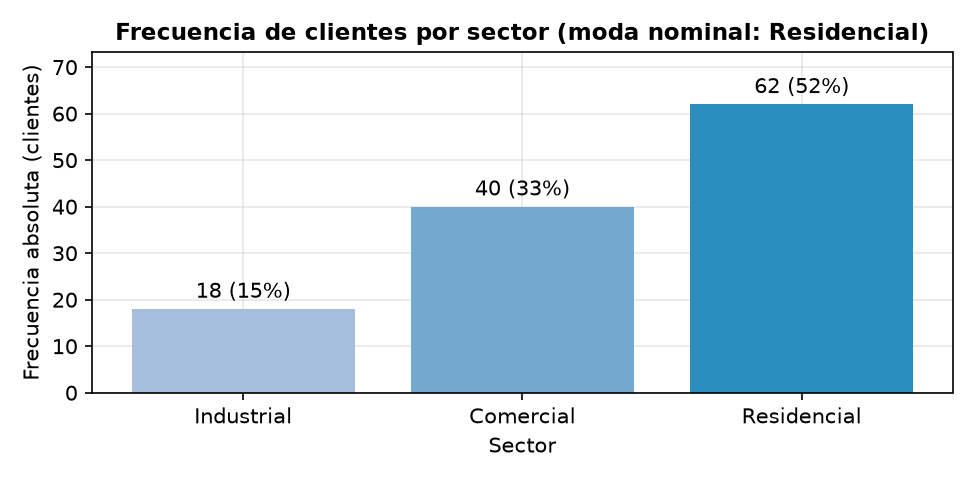
\includegraphics[width=0.45\linewidth]{assets/images/figures/python/bar_freq_by_sector.png}
            \hfill
            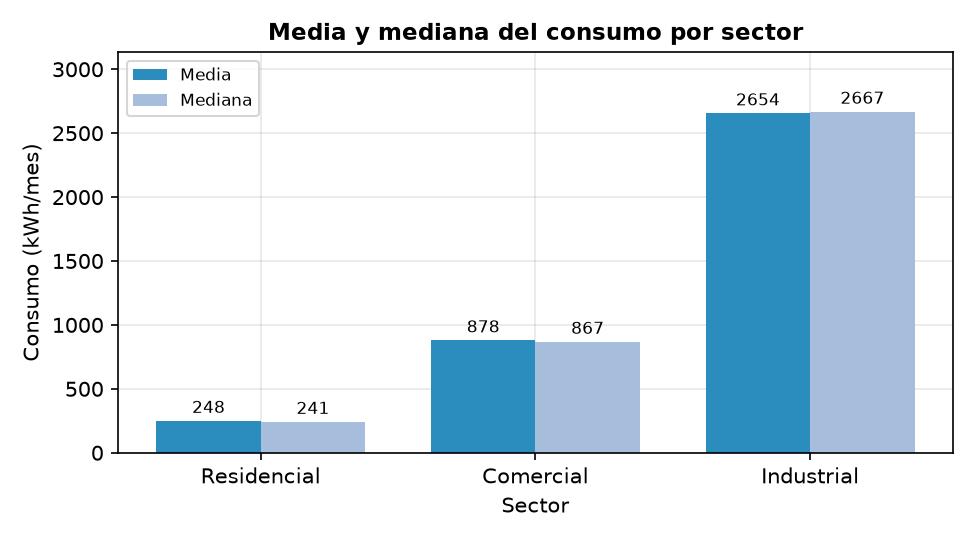
\includegraphics[width=0.45\linewidth]{assets/images/figures/python/bar_mean_median_by_sector.png}

            \vspace{6pt}

            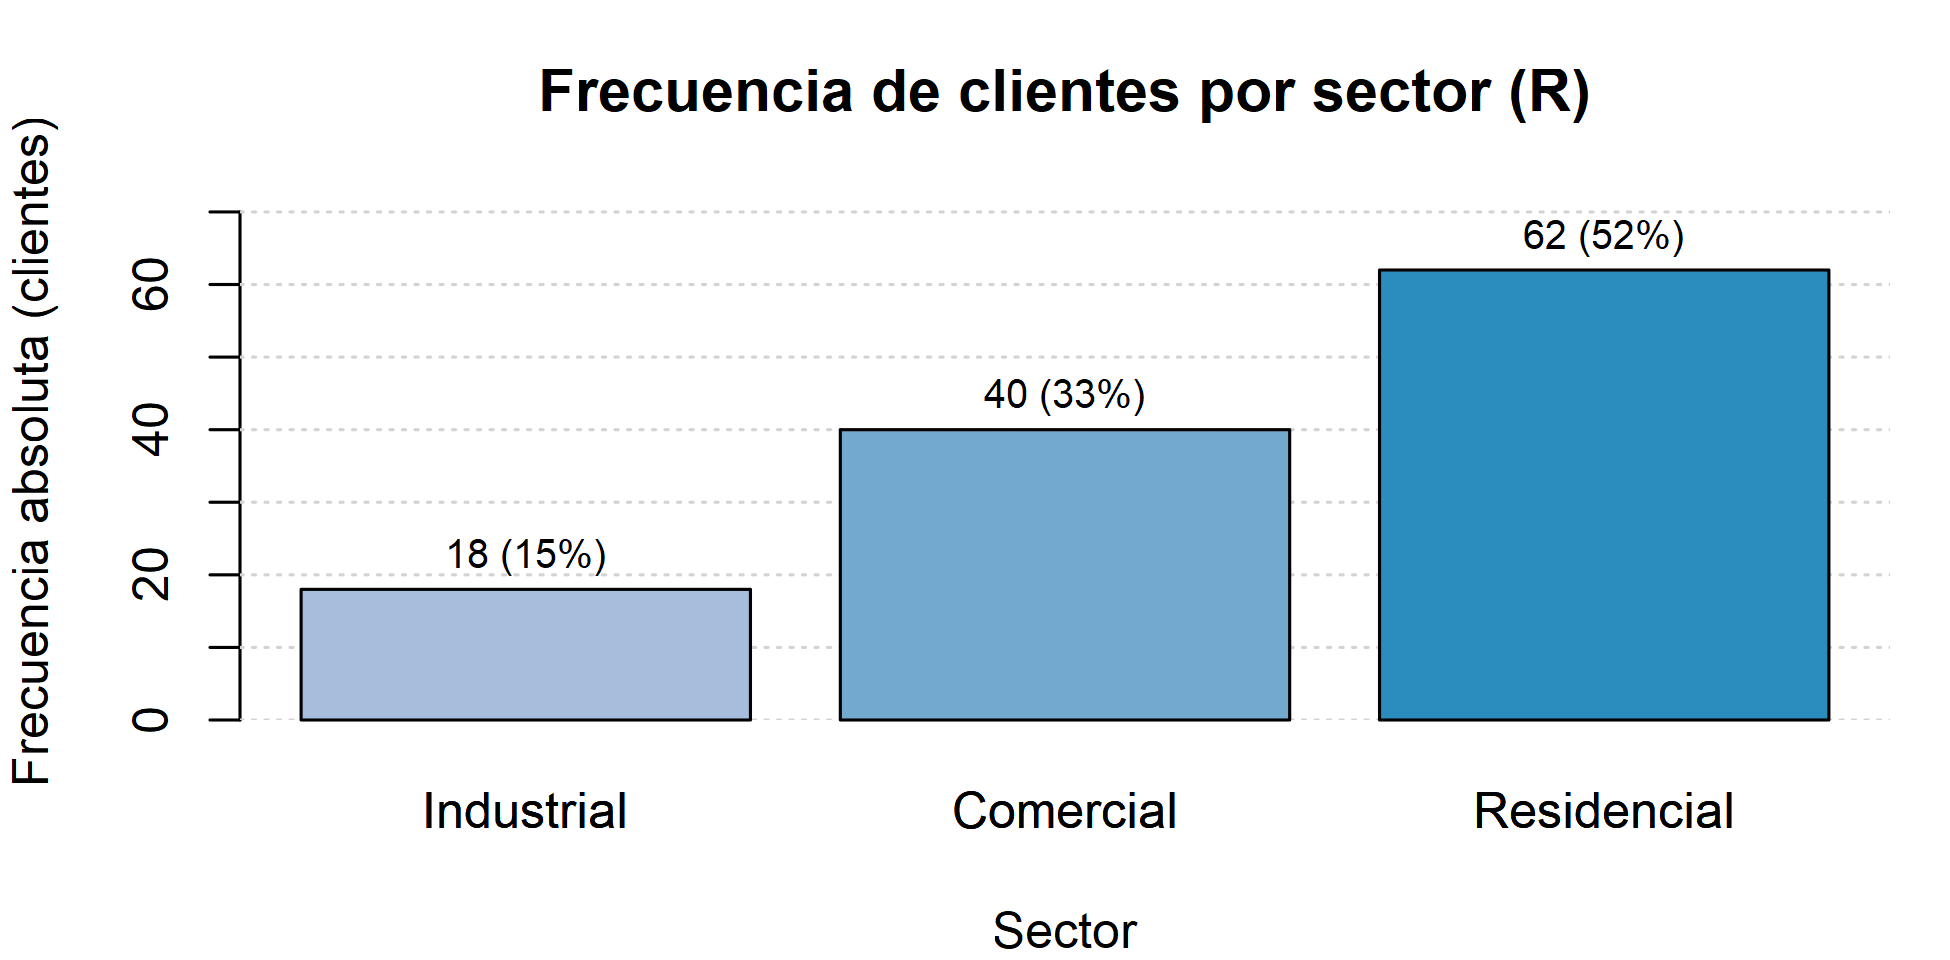
\includegraphics[width=0.45\linewidth]{assets/images/figures/r/bar_freq_by_sector.png}
            \hfill
            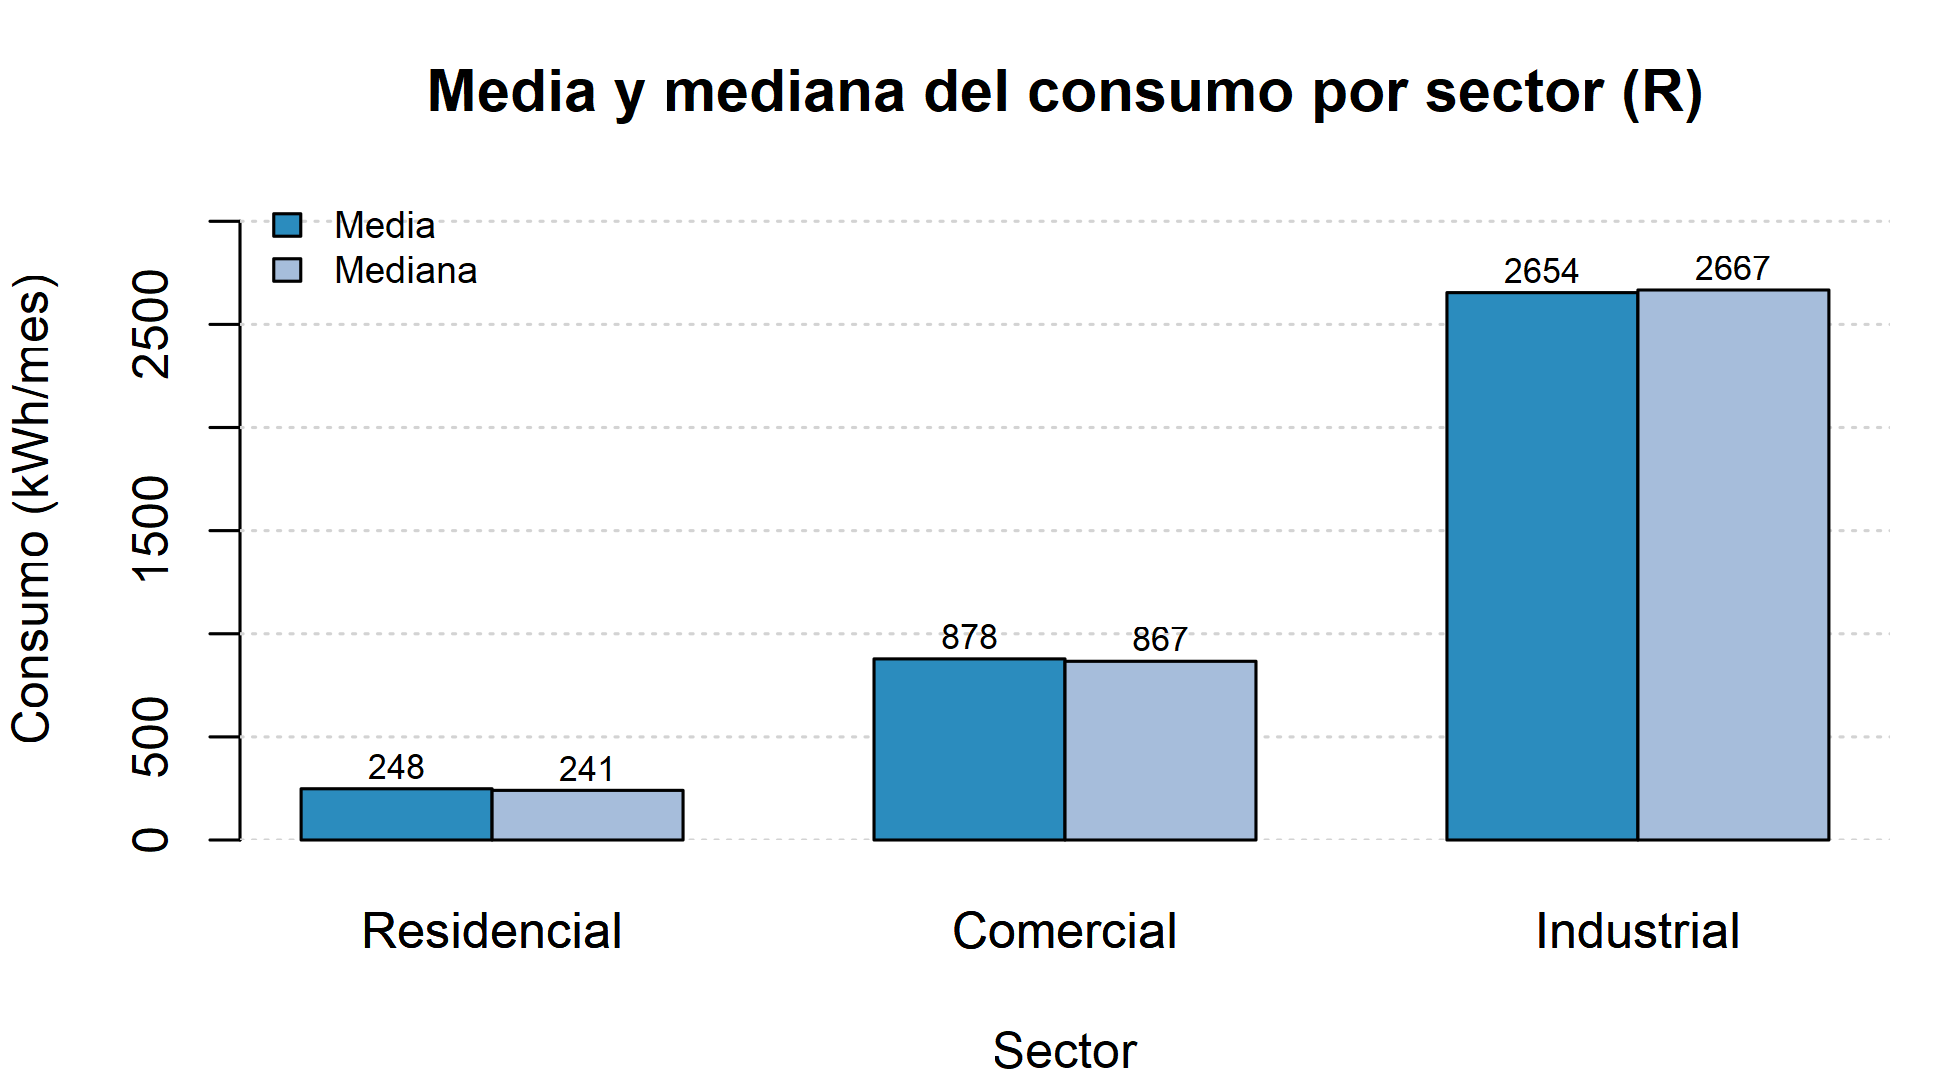
\includegraphics[width=0.45\linewidth]{assets/images/figures/r/bar_mean_median_by_sector.png}

            \vspace{4pt}

            \captionof{figure}{Frecuencia de clientes por sector con la moda nominal
            Residencial (izquierda) y comparación entre media y mediana por sector
            (derecha), en Matplotlib (arriba) y su réplica en R (abajo)}
            \label{bar_sector}
        \end{strip}

    \subsection{Medidas de dispersión}
        La Tabla \ref{dispersion} presenta las medidas de dispersión del consumo por
        sector y a nivel global, y la Figura \ref{boxplot_dispersion} las representa
        mediante el diagrama de caja con la media y la desviación estándar superpuestas.

        \begin{table}[H]
            \centering
            \caption{Medidas de dispersión del consumo mensual (kWh)}
            \begin{center}
                \begin{tabular}{|l|c|c|c|c|c|}
                    \hline
                    \textbf{Grupo} & \textbf{Rango} & \textbf{Varianza} &
                    $\mathbf{s}$ & \textbf{CV (\%)} & \textbf{IQR} \\
                    \hline
                    Residencial & 303,6   & 3.736,3   & 61,1  & 24,6  & 69,5    \\
                    \hline
                    Comercial   & 908,4   & 42.989,5  & 207,3 & 23,6  & 255,3   \\
                    \hline
                    Industrial  & 2.103,1 & 471.785,8 & 686,9 & 25,9  & 1.322,8 \\
                    \hline
                    Global      & 3.655,9 & 763.564,7 & 873,8 & 106,7 & 742,0   \\
                    \hline
                \end{tabular}
                \label{dispersion}
            \end{center}
        \end{table}

        Con el fin de representar las cifras obtenidas en su forma gráfica, la Figura
        \ref{boxplot_dispersion} traduce los valores de la Tabla \ref{dispersion} en el
        diagrama de caja, que resume en una sola imagen la posición de la mediana, la
        amplitud del rango intercuartílico y el alcance de los bigotes, con la media y la
        desviación estándar superpuestas en cada grupo, junto con su réplica en R, de
        esta manera, la brecha de escala entre sectores y la homogeneidad de su
        dispersión relativa, que en la tabla se leen número a número, se aprecian de un
        solo vistazo.

        \begin{figure}[H]
            \centering
            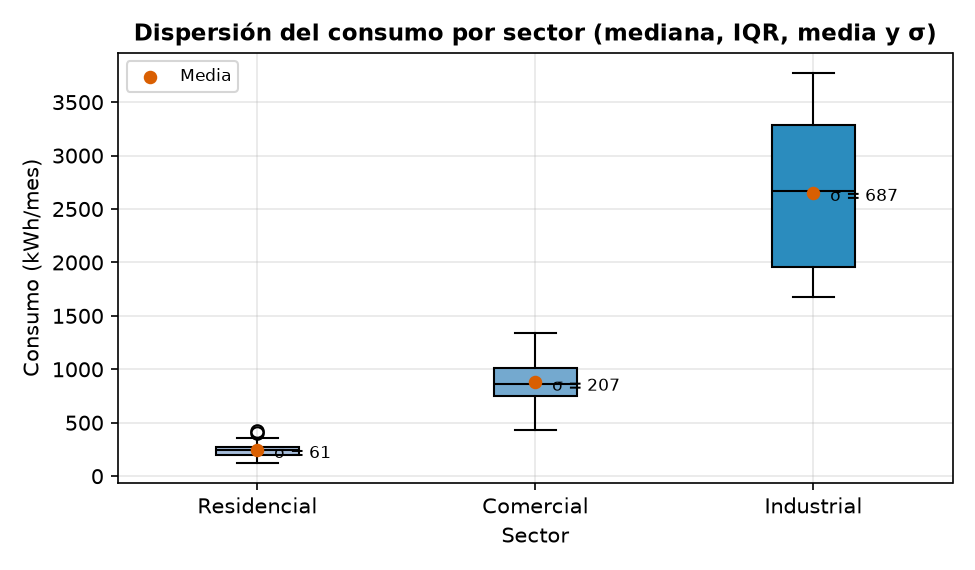
\includegraphics[width=1\linewidth]{assets/images/figures/python/boxplot_dispersion_by_sector.png}

            \vspace{4pt}

            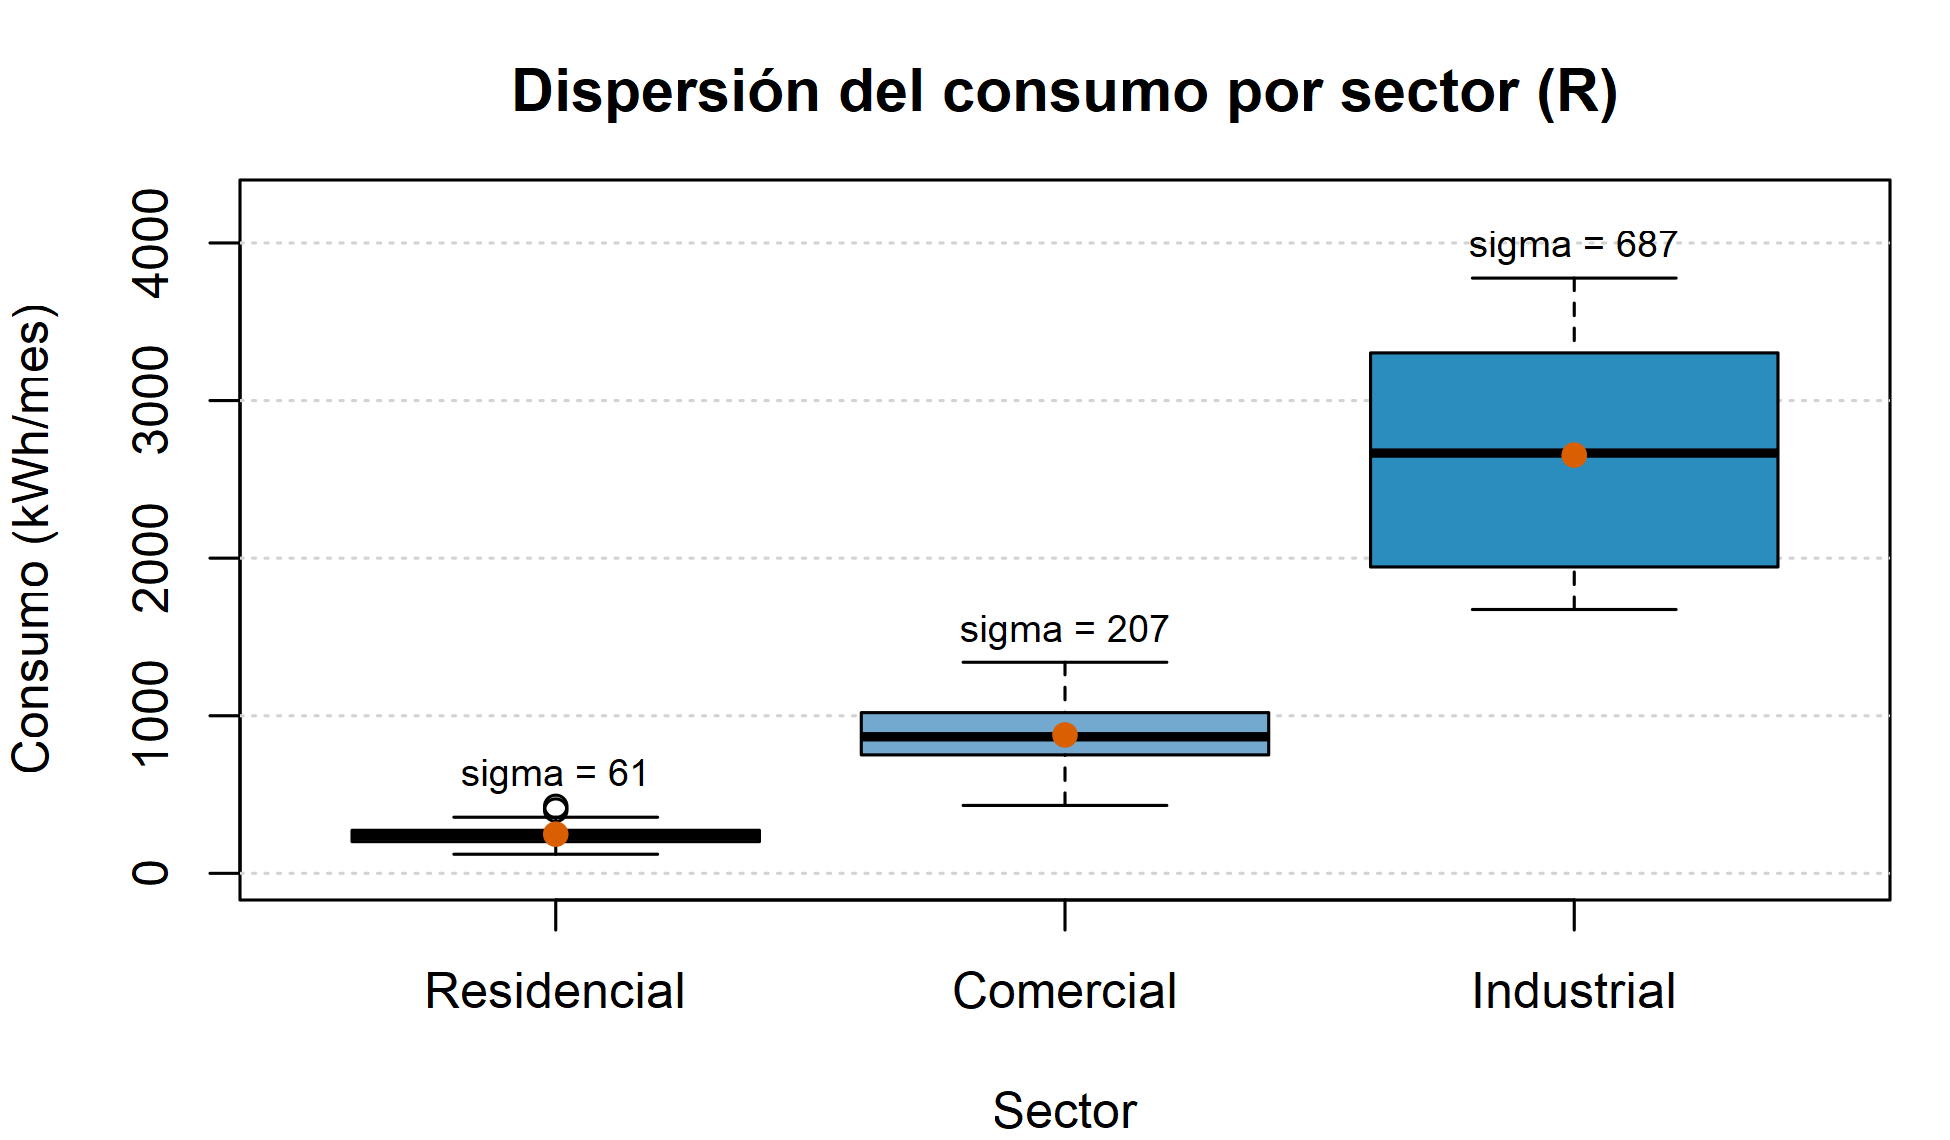
\includegraphics[width=1\linewidth]{assets/images/figures/r/boxplot_dispersion_by_sector.png}
            \caption{Dispersión del consumo por sector con mediana, IQR, media y
            $\sigma$, en Matplotlib (arriba) y su réplica en R (abajo)}
            \label{boxplot_dispersion}
        \end{figure}

        La lectura conjunta de la tabla y la figura arroja tres deducciones, la primera,
        que la dispersión absoluta crece con la escala del sector, pues la desviación
        estándar pasa de 61,1 kWh en Residencial a 686,9 kWh en Industrial y la varianza
        amplifica esa brecha en dos órdenes de magnitud, lo que en el diagrama de caja se
        aprecia como cajas y bigotes progresivamente más amplios, la segunda radica en
        que la dispersión relativa resulta homogénea, ya que el coeficiente de variación
        se mantiene entre 23,6\% y 25,9\% en los tres sectores, es decir, cada grupo
        es igualmente variable en proporción a su media y la tercera, que el CV global
        (106,7\%) cuadruplica al de cualquier sector, una explosión de variabilidad
        relativa que no proviene de la dispersión interna de los grupos sino de la
        distancia entre sus centros, lo que constituye la evidencia numérica de que el
        conjunto global es una mezcla de poblaciones, en plena coherencia con el vacío de
        la Tabla \ref{freq_table} y la separación sin traslape de las cajas en la Figura
        \ref{boxplot_dispersion}.

    \subsection{Verificación cruzada entre Python y R}
        El script de R recalculó de forma independiente la tabla de frecuencias completa,
        con las mismas ocho clases donde las medidas de tendencia central, incluida la
        moda interpolada por clase modal y las medidas de dispersión coinciden dígito a
        dígito con los resultados de Python, por ende, se puede concluir que la
        equivalencia entre \texttt{var()} y \texttt{sd()} de R y el parámetro
        \texttt{ddof=1} de pandas explica la coincidencia exacta de las varianzas
        muestrales. Las réplicas gráficas en sus paneles de R conservan además los
        principios de diseño, con la cuadrícula trazada en dos pasadas, confirmando que
        tanto los cálculos como su representación son independientes de la herramienta
        empleada.


    \section{Conclusiones}
    \begin{itemize}
        \item La distribución de frecuencias construida con la regla de Sturges resume
        en ocho clases la estructura del consumo donde el 54,2\% de los clientes cae
        en la primera clase, el 76,7\% se acumula por debajo de 1.035,2 kWh y el vacío
        entre 1.949,2 y 2.406,1 kWh delata la existencia de subpoblaciones separadas,
        hecho que el cruce con el sector confirma, pues cada clase agrupa casi
        exclusivamente a clientes de un mismo sector, información que ninguna medida
        resumen entrega por sí sola.

        \vspace{10pt}

        \item La relación entre las tres medidas de tendencia central funciona como
        diagnóstico de forma, puesto que a nivel global la media (819,1 kWh) supera
        ampliamente a la mediana (378,6 kWh) y a la moda interpolada (409,6 kWh), firma
        de una asimetría positiva pronunciada, mientras que dentro de cada sector media
        y mediana casi coinciden, evidencia de simetría local.

        \vspace{10pt}

        \item La media global no describe a ningún cliente típico, pues su discrepancia
        con la mediana no obedece a valores atípicos sino a la mezcla de tres poblaciones
        con escalas distintas, por lo que todo análisis operativo del consumo debe
        segmentarse por sector antes de promediar.

        \vspace{10pt}

        \item Las medidas de dispersión cuentan la misma historia desde la variabilidad,
        ya que la desviación estándar crece con la escala del sector, pasando de 61,1 a
        207,3 y a 686,9 kWh, pero el coeficiente de variación permanece homogéneo entre
        23,6\% y 25,9\%, y su salto a 106,7\% en el agregado global cuantifica que
        la variabilidad del conjunto proviene de la distancia entre los centros de los
        grupos y no de la dispersión interna.

        \vspace{10pt}

        \item Los gráficos básicos son la contraparte visual exacta de cada cálculo,
        puesto que el histograma y el polígono materializan la tabla de frecuencias, la
        ojiva permite leer la mediana en el 50\% acumulado, el diagrama de barras
        describe la variable nominal y contrasta media con mediana en cada sector, y el
        diagrama de caja integra mediana, IQR, media y desviación
        estándar en una sola figura, de modo que estadístico y gráfico se validan
        mutuamente.

        \vspace{10pt}

        \item La verificación cruzada entre pandas con Matplotlib y R base, con
        coincidencia dígito a dígito de todos los estadísticos gracias a la equivalencia
        entre \texttt{var()} y \texttt{sd()} de R y el parámetro \texttt{ddof=1} de
        pandas, confirma la corrección de la implementación y muestra que el análisis
        descriptivo y sus principios de representación son independientes de la
        herramienta.
    \end{itemize}


    \appendices
    \section{Código en Python}
    \label{anexo_python}
    Las fases 0 a 4 de la Tabla \ref{workflow} se implementan en Python y se
    reproducen completas a continuación, en su orden de ejecución.

    \subsection{\textit{dataset.py}}
        Regenera el conjunto de datos con la semilla fija 42 y añade la variable
        derivada \texttt{tarifa\_cop\_kwh} de la Tabla \ref{dataset_variables}, que
        después sirve como patrón externo contra el cual contrastar las pendientes
        estimadas.

        \vspace{10pt}

        \lstinputlisting[style=python]{utils/codes/python/dataset.py}

    \subsection{\textit{simple\_regression.py}}
        Calcula las correlaciones de la Tabla \ref{correlations}, estima el modelo M1
        de la Tabla \ref{coef_m1}, aplica las cuatro pruebas de supuestos de la Tabla
        \ref{diagnostics_m1}, cuantifica el sesgo por sector de la Tabla
        \ref{sector_bias} y produce las Figuras \ref{fit_m1}, \ref{diag_panel} y
        \ref{bias_boxplot}.

        \vspace{10pt}

        \lstinputlisting[style=python]{utils/codes/python/simple_regression.py}

    \subsection{\textit{multiple\_regression.py}}
        Estima los modelos M2 y M3, ejecuta el contraste F de la Tabla \ref{anova},
        traduce las pendientes a las tarifas de la Tabla \ref{tariffs}, compara los
        tres modelos en la Tabla \ref{model_comparison} y genera las Figuras
        \ref{fit_m3}, \ref{coef_plot} y \ref{criteria}.

        \vspace{10pt}

        \lstinputlisting[style=python]{utils/codes/python/multiple_regression.py}

    \subsection{\textit{ml\_regression.py}}
        Construye la partición estratificada y la validación cruzada de diez pliegues
        dentro de un \texttt{Pipeline}, produciendo la Tabla \ref{ml_validation} y la
        Figura \ref{holdout}.

        \vspace{10pt}

        \lstinputlisting[style=python]{utils/codes/python/ml_regression.py}

    \subsection{\textit{advanced\_viz.py}}
        Lee las tablas que dejó la fase 2 en lugar de recalcularlas y construye las
        cuatro figuras de \textit{seaborn} (\ref{heatmap}, \ref{scatter_matrix},
        \ref{lmplot} y \ref{lowess}) y las dos piezas interactivas de \textit{Plotly}
        (\ref{dashboard} y \ref{scatter_plotly}).

        \vspace{10pt}

        \lstinputlisting[style=python]{utils/codes/python/advanced_viz.py}

    \section{Código en R}
    \label{anexo_r}
    El script \textit{statistics.R} implementa la verificación cruzada. Lee el mismo
    archivo CSV, recalcula de forma independiente la distribución de frecuencias y todos
    los estadísticos de las Tablas \ref{freq_table} a \ref{dispersion}, y replica los
    gráficos básicos con la graficación base de R, trazando la cuadrícula en dos pasadas
    para mantenerla detrás de los datos. Se reproduce completo a continuación, con los
    mismos bloques del Anexo \ref{anexo_python} para que la comparación entre ambas
    implementaciones sea directa.

    \vspace{10pt}

    \lstinputlisting[style=rlang]{utils/codes/full/statistics.R}


    \bibliographystyle{IEEEtran}
    \bibliography{utils/references/references.bib}

\end{document}
